\documentclass[11pt]{article}
\usepackage{amsmath,amssymb}
\usepackage[makeroom]{cancel}
\usepackage{graphicx}
\usepackage{array}
\usepackage{changes}
\usepackage{natbib}
\graphicspath{ ../figs/}
\usepackage[margin=1in]{geometry}
\usepackage[parfill]{parskip}  
\title{Southwest US drought dynamics \large \\}
\author{Daniel Kennedy - djk2120@ucar.edu \\ Isla Simpson }

\begin{document}
\maketitle

\section{Introduction}

\begin{itemize}
    \item SWUS experienced a megadrought, and 2020 was the driest year on record.
    \item The 2020 drought was associated with xyz
    \item Climate change is not understood to have greatly exacerbated the 2020 drought.
    \item Whether average precipitation is projected to increase, decrease, or remain the same varies among climate models
    \item CESM2 projects that average precipitation will stay the same
    \item The statistics of determining whether extreme events are getting more extreme is more tenuous given the smaller sample size.
\end{itemize}


\begin{figure}[h]
\centering
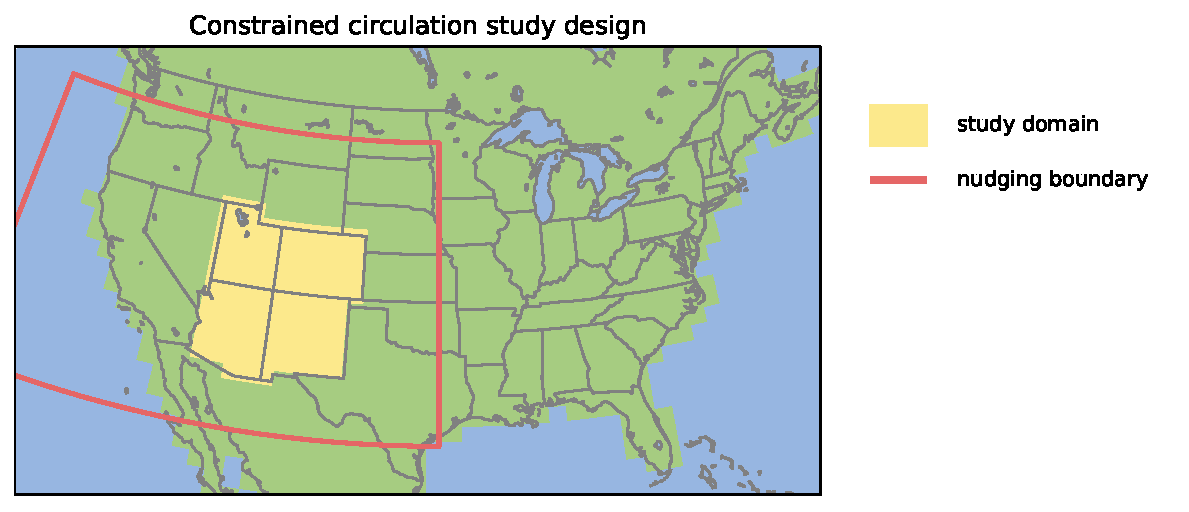
\includegraphics[width=40pc]{figs/domain.pdf}
\caption{Map of our study domain (yellow) and the nudging box (red).}
\label{fig:domain}
\end{figure}


\newpage

\begin{figure}[h]
\centering
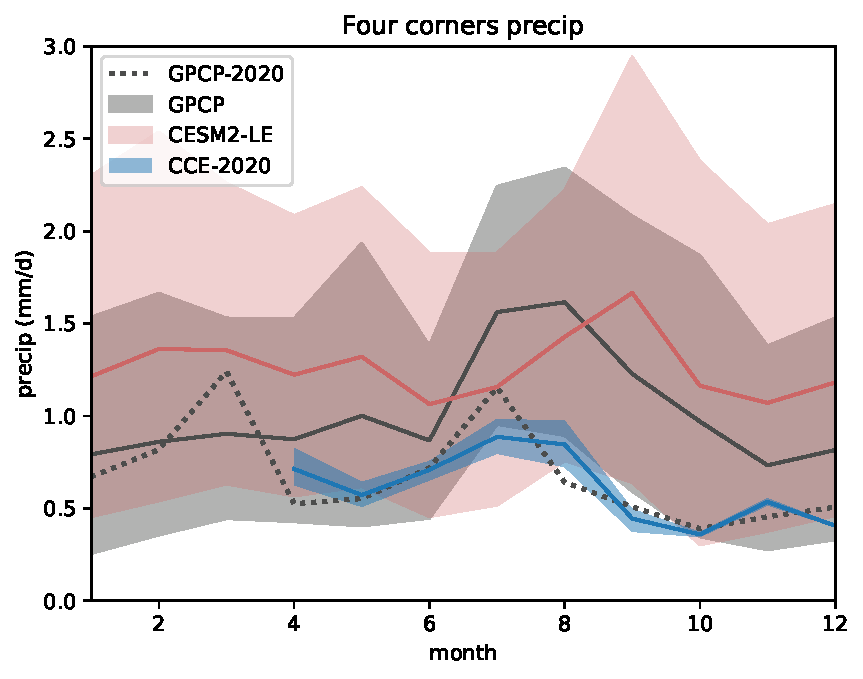
\includegraphics[width=25pc]{figs/main/precip.pdf}
\caption{Precip in the four corners.}
\label{fig:precip}
\end{figure}


\newpage

\begin{figure}[h]
\centering
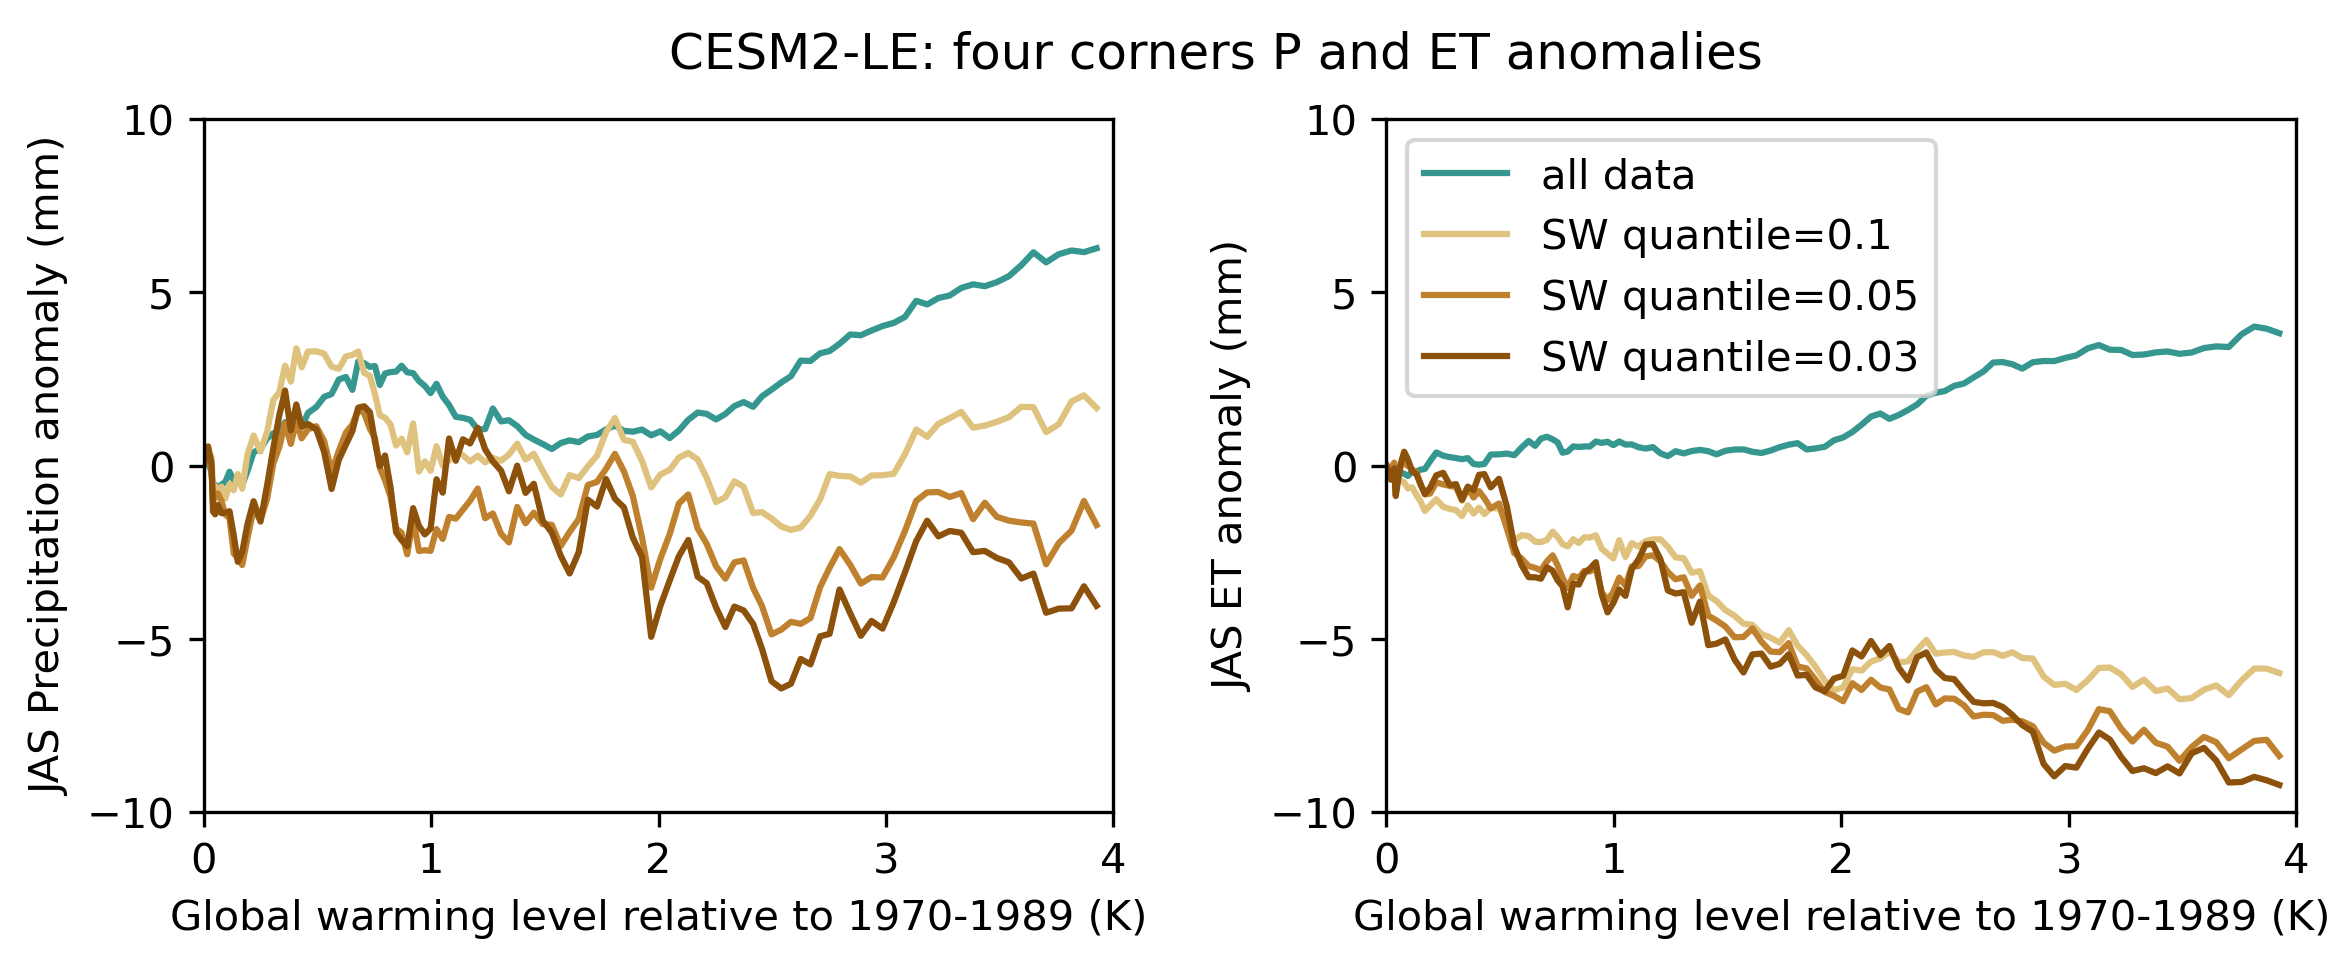
\includegraphics[width=40pc]{figs/main/anomalies.png}
\caption{Anomalies w/r/t warming in the four corners.}
\label{fig:anomalies}
\end{figure}


\newpage
\begin{figure}[h]
\centering
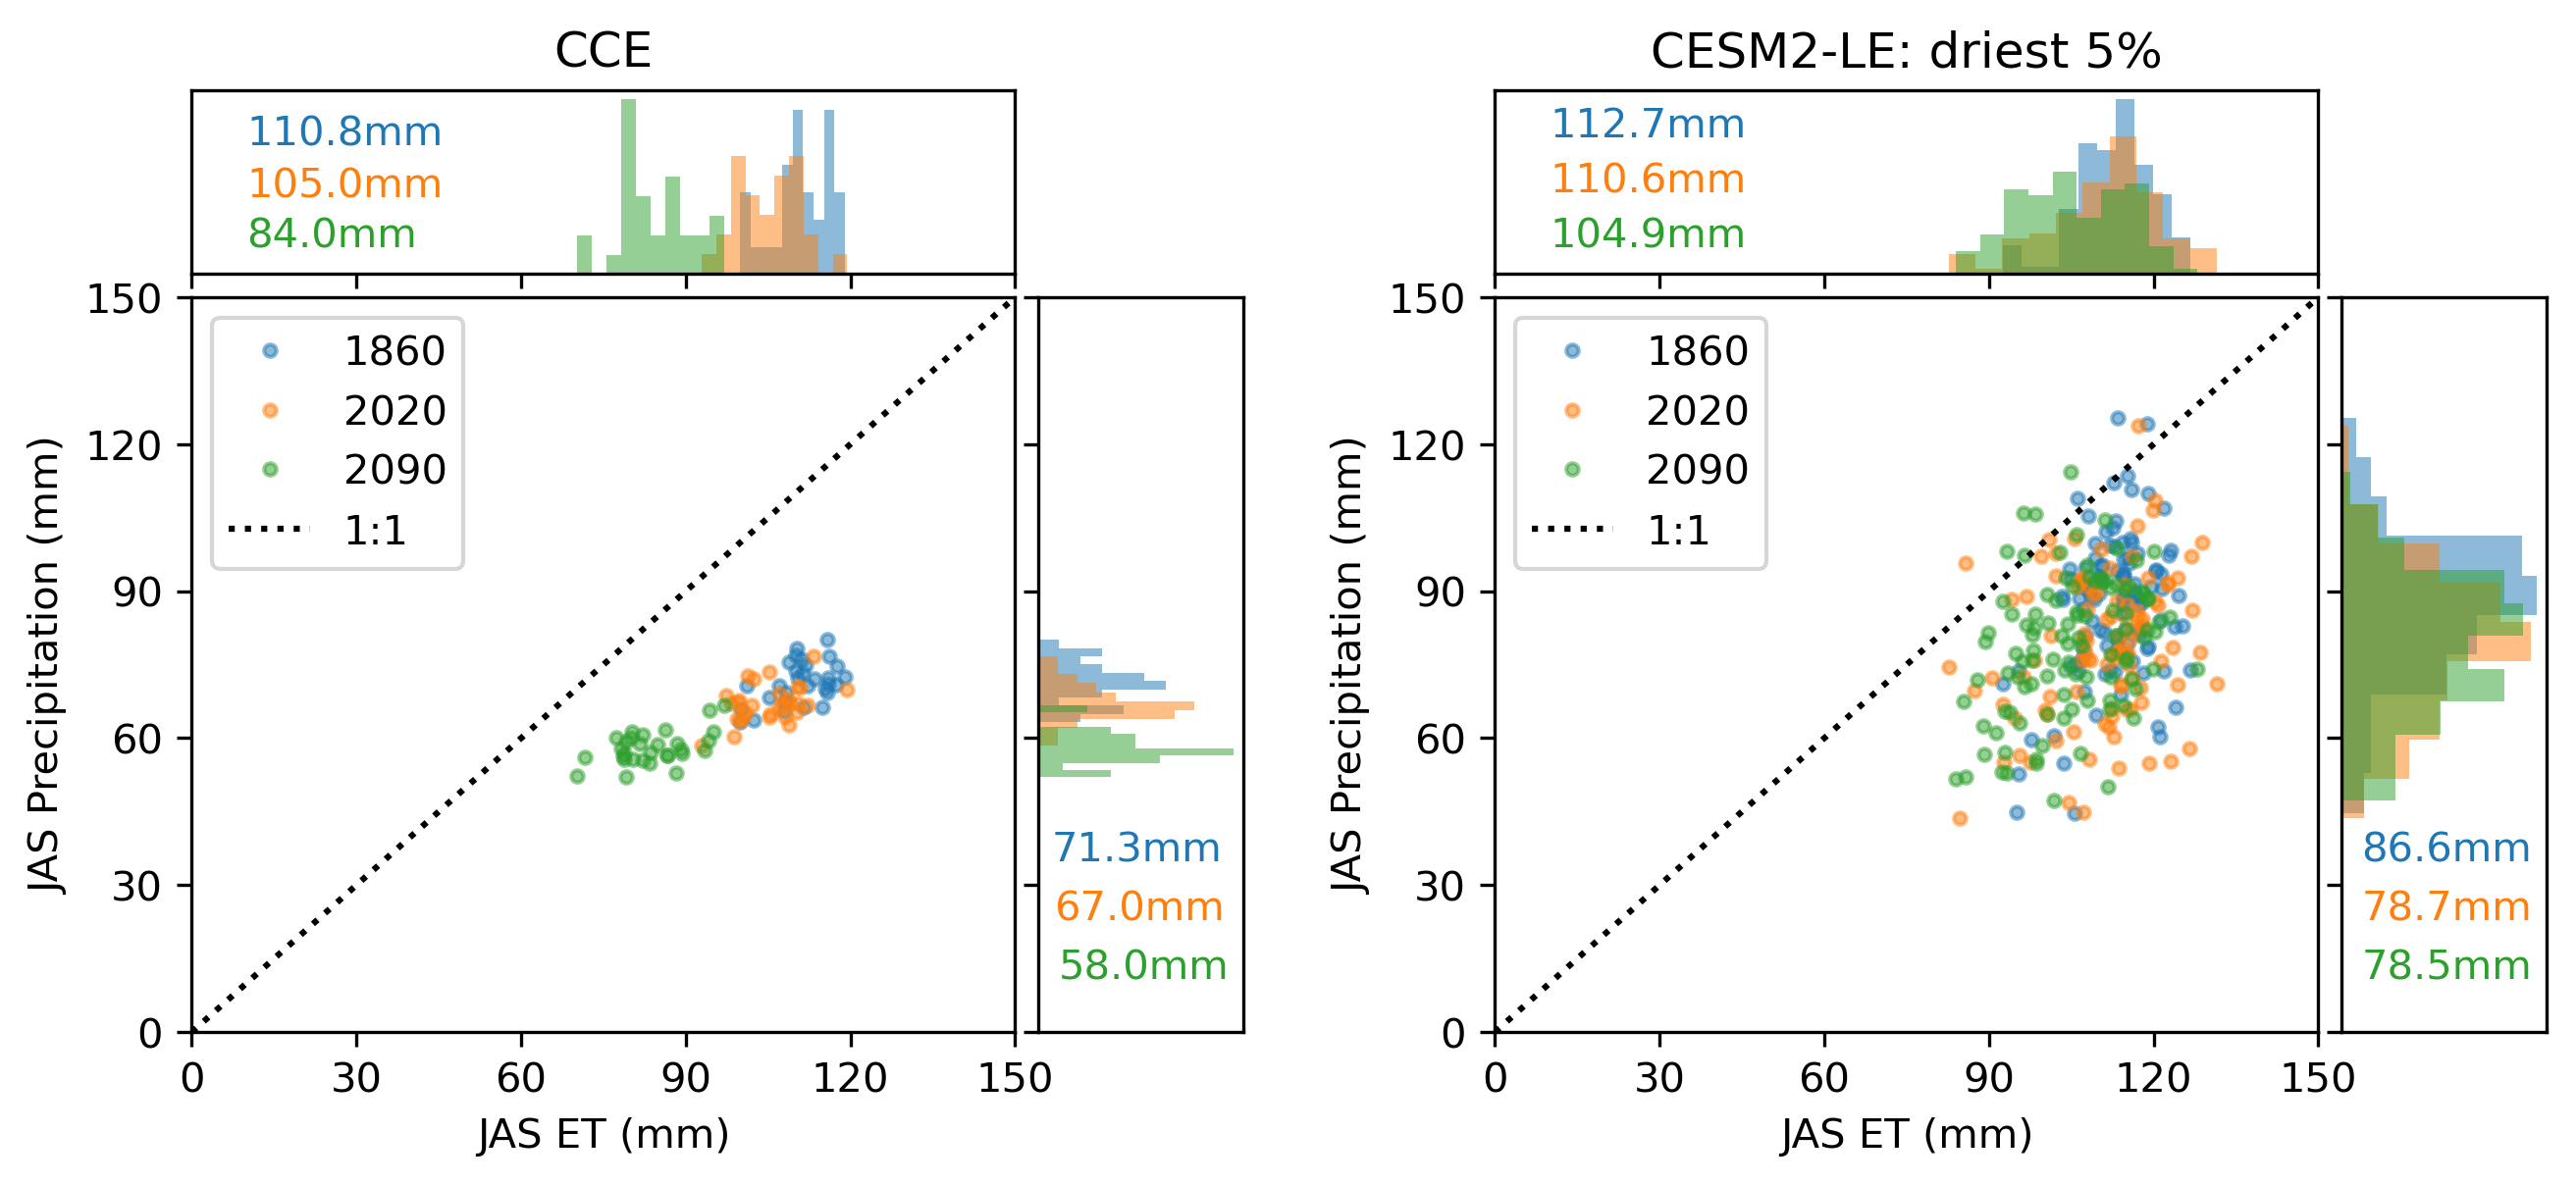
\includegraphics[width=40pc]{figs/main/scatter_ET_P.png}
\caption{Precipitation vs. ET in the constrained ensemble and the driest 3\% of the large ensemble.}
\label{fig:precip}
\end{figure}



SWUS JAS Rain and ET in these ensembles:
\begin{itemize}
    \item In the CCE: precip and ET decrease with warming.
    \item In CESM2-LE on average, precip is highest in 1850, lowest in 2020, and in between those two in 2090.
    \item In CESM2-LE dry composites, 1850 has more rain, 2020 and 2090 are not distinguishable
    \item In CESM2-LE on average, ET increases with warming.
    \item In CESM2-LE, evaporation \textbf{decreases} with warming in all of the dry composites    
\end{itemize}


\begin{figure}[h]
\centering
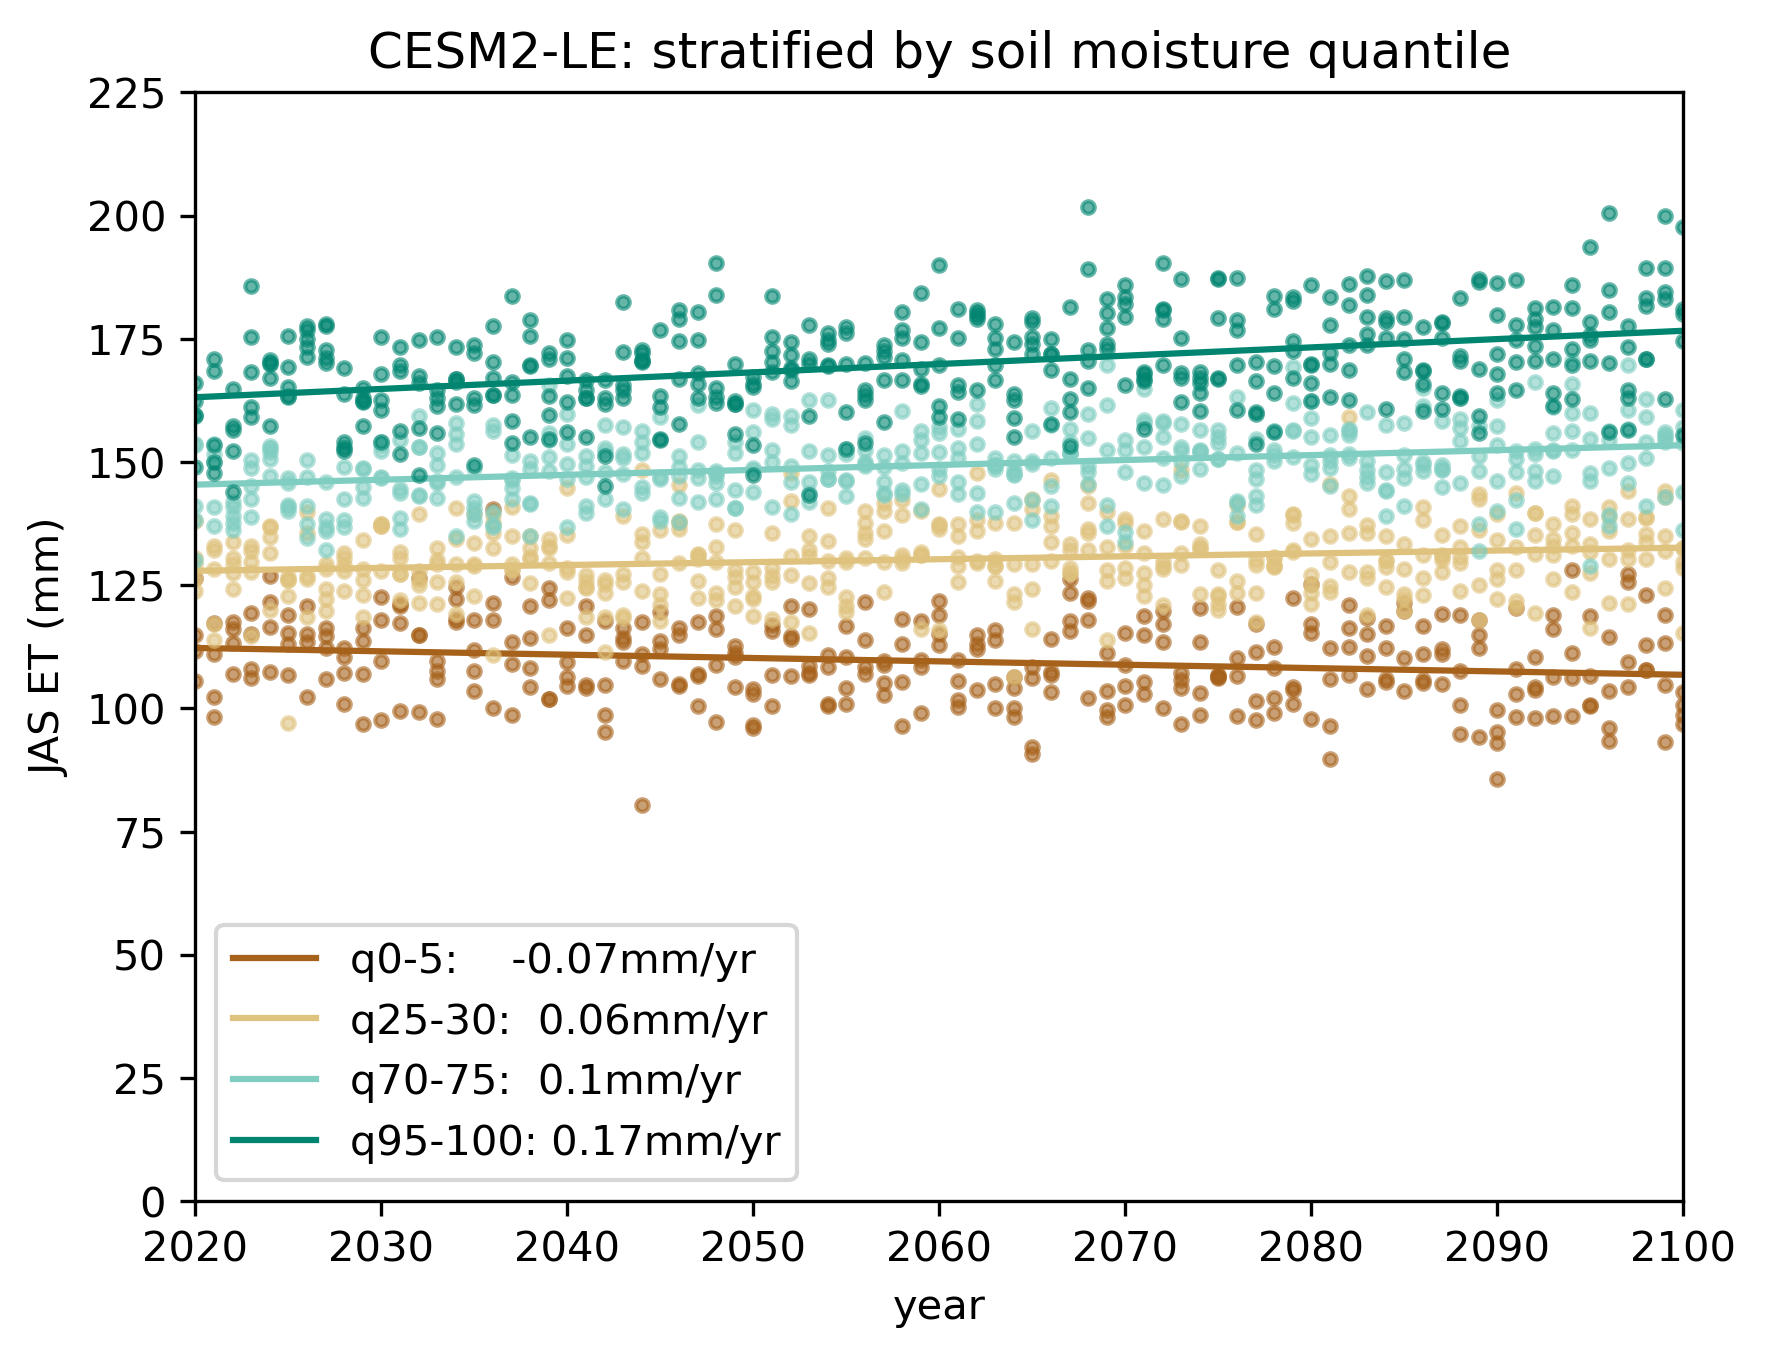
\includegraphics[width=25pc]{figs/supp/et_trends.png}
\caption{[SUPP] ET increases in most cases, but decreases in the driest SW10cm quantiles.}
\label{fig:precip}
\end{figure}


\begin{figure}[h]
\centering
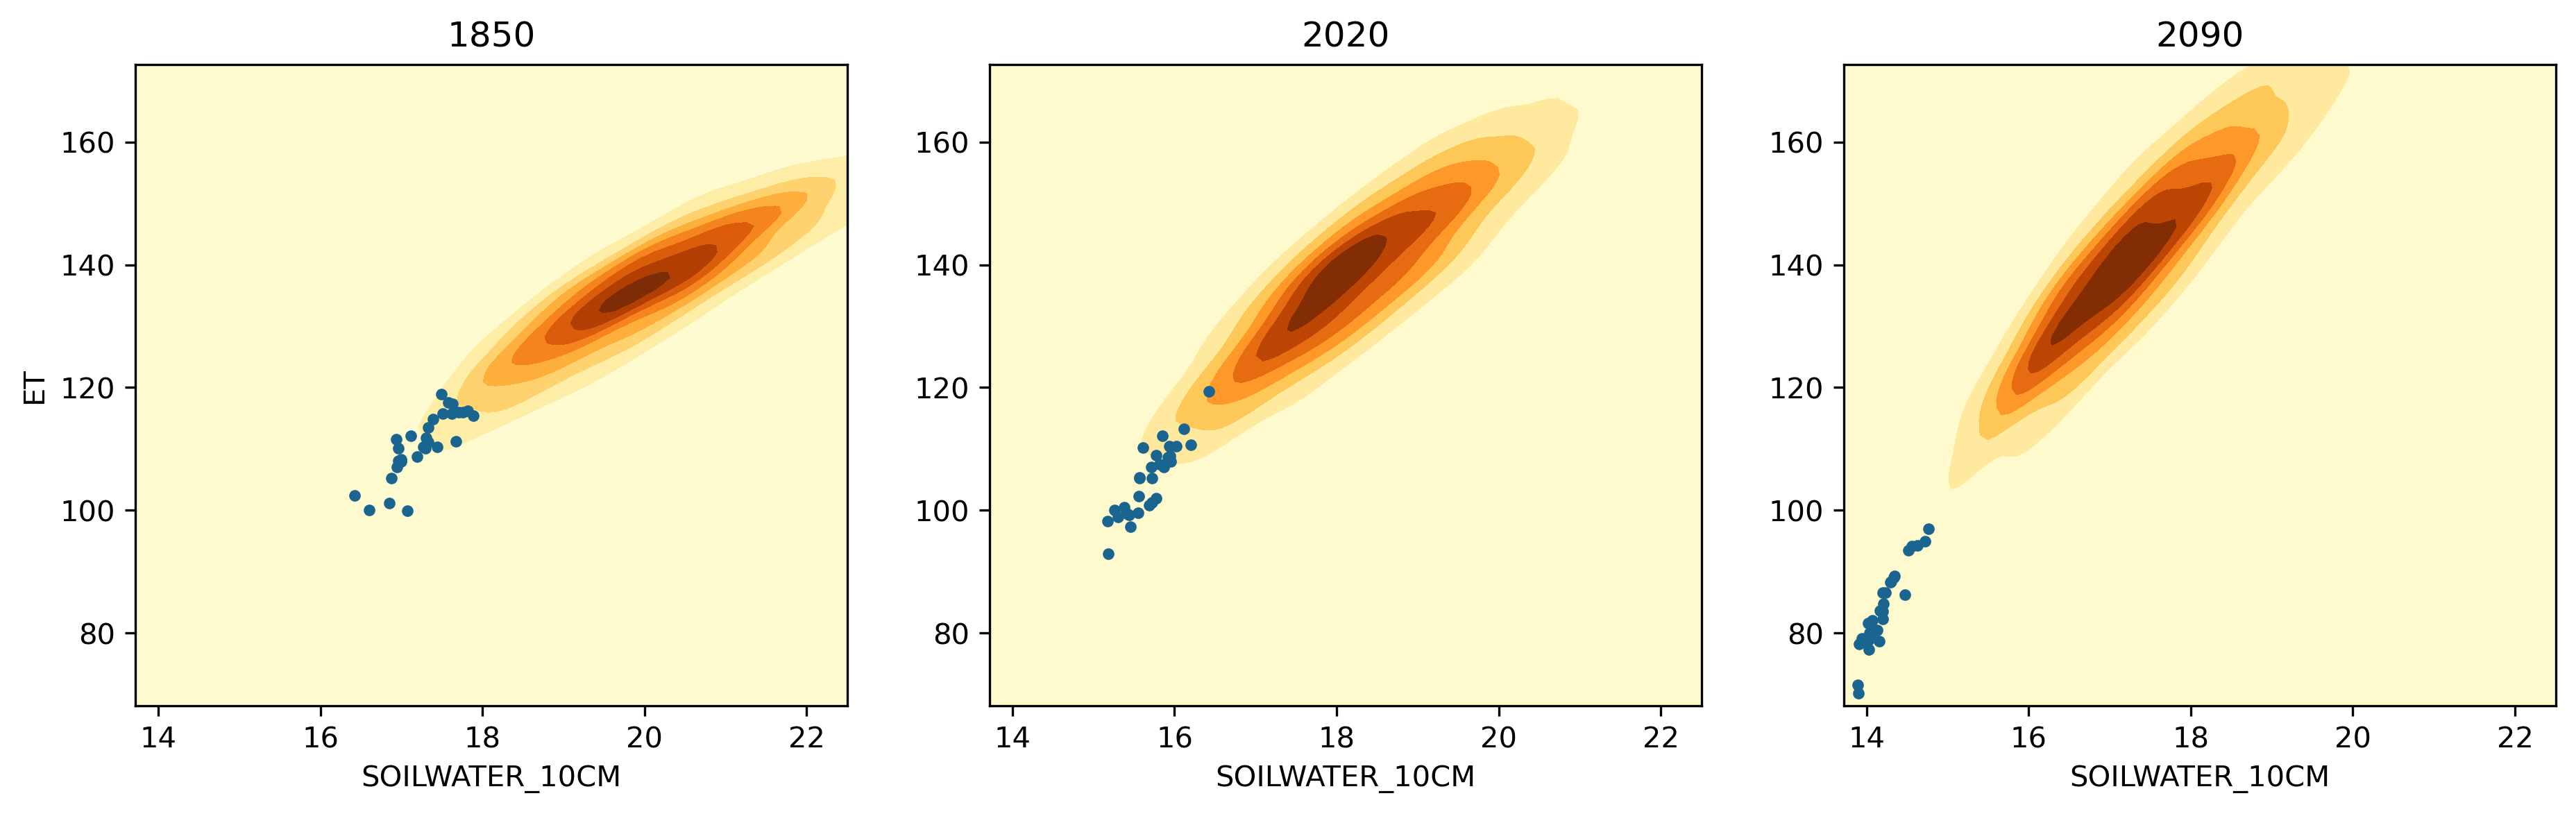
\includegraphics[width=40pc]{figs/contours/SOILWATER_10CM_ET_contours.png}
\caption{[MAIN] The CCE ET$\sim$SW relationship seems consistent with the large ensemble.}
\label{fig:precip}
\end{figure}

\begin{figure}[h]
\centering
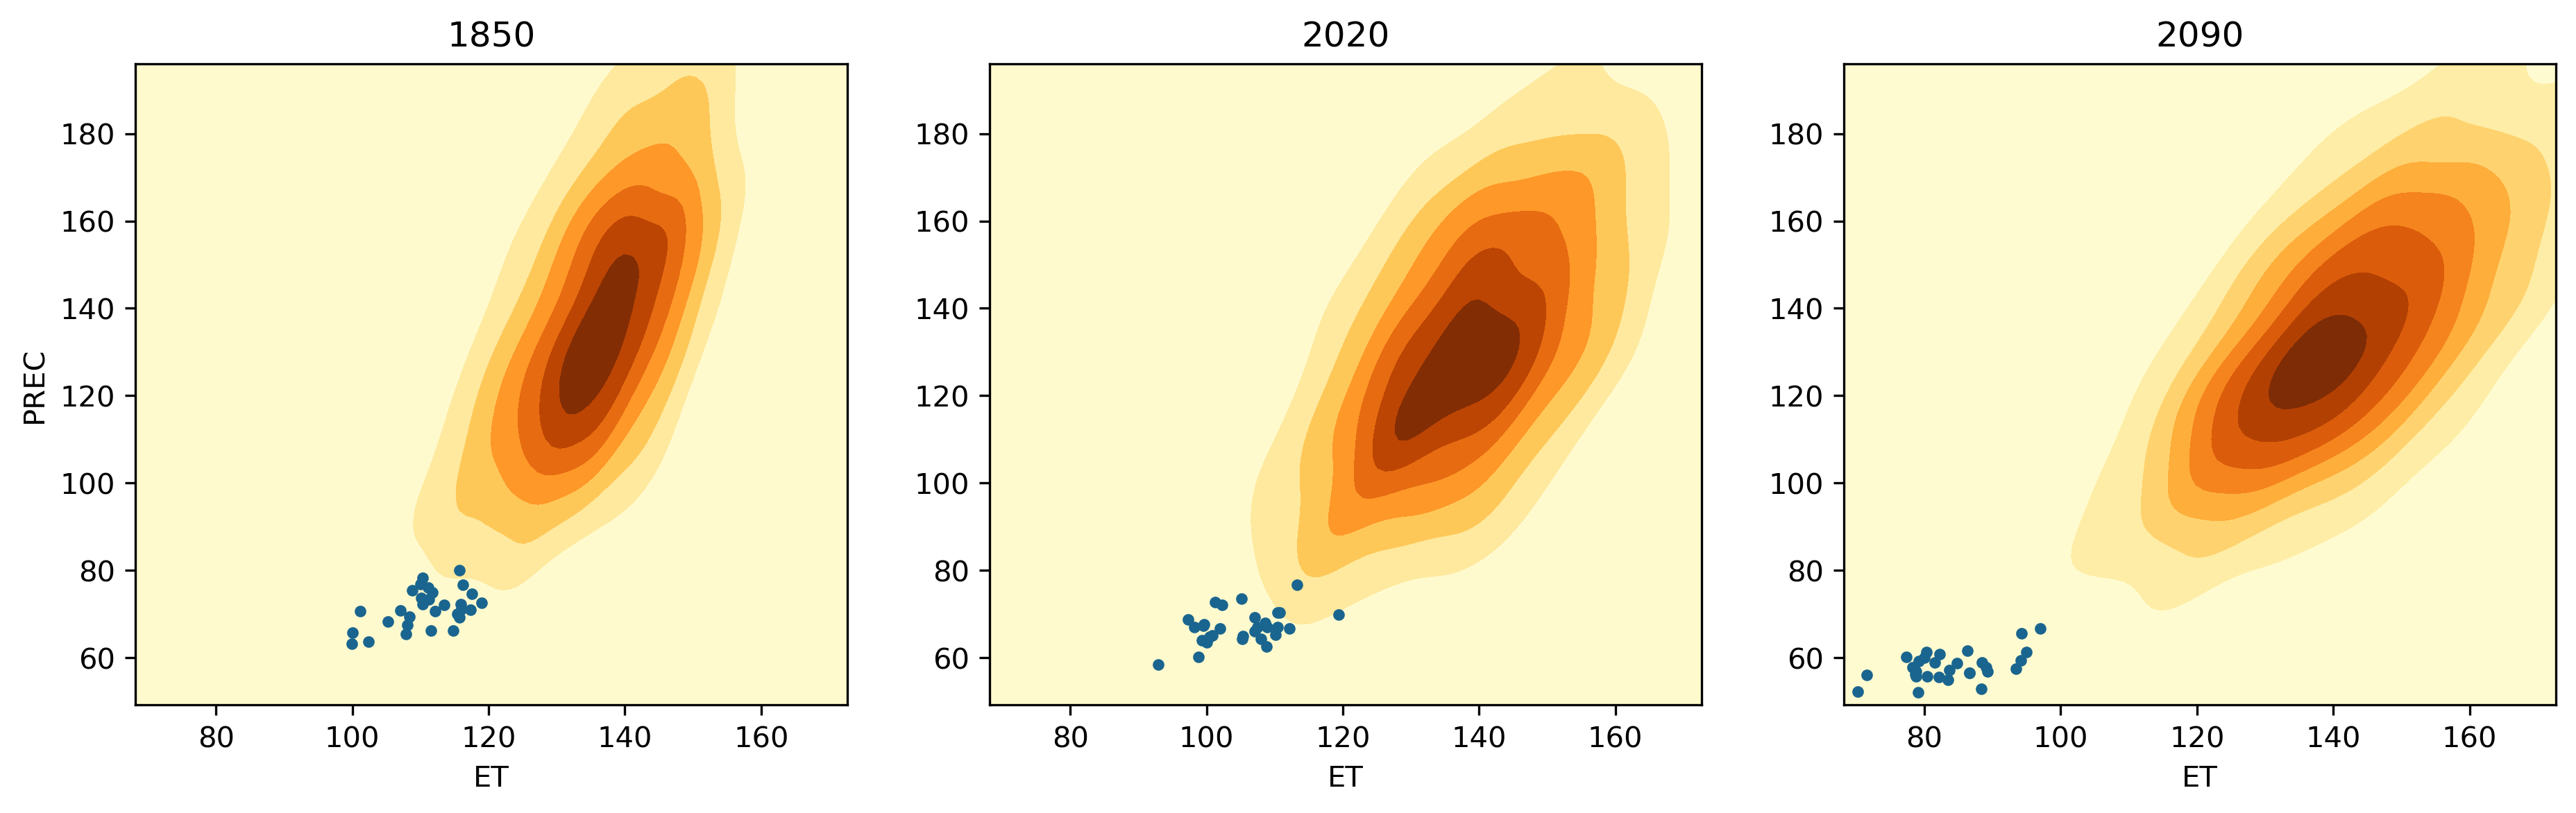
\includegraphics[width=40pc]{figs/contours/ET_PREC_contours.png}
\caption{[SUPP] The CCE P$\sim$ET seems somewhat different.}
\label{fig:precip}
\end{figure}

\begin{figure}[h]
\centering
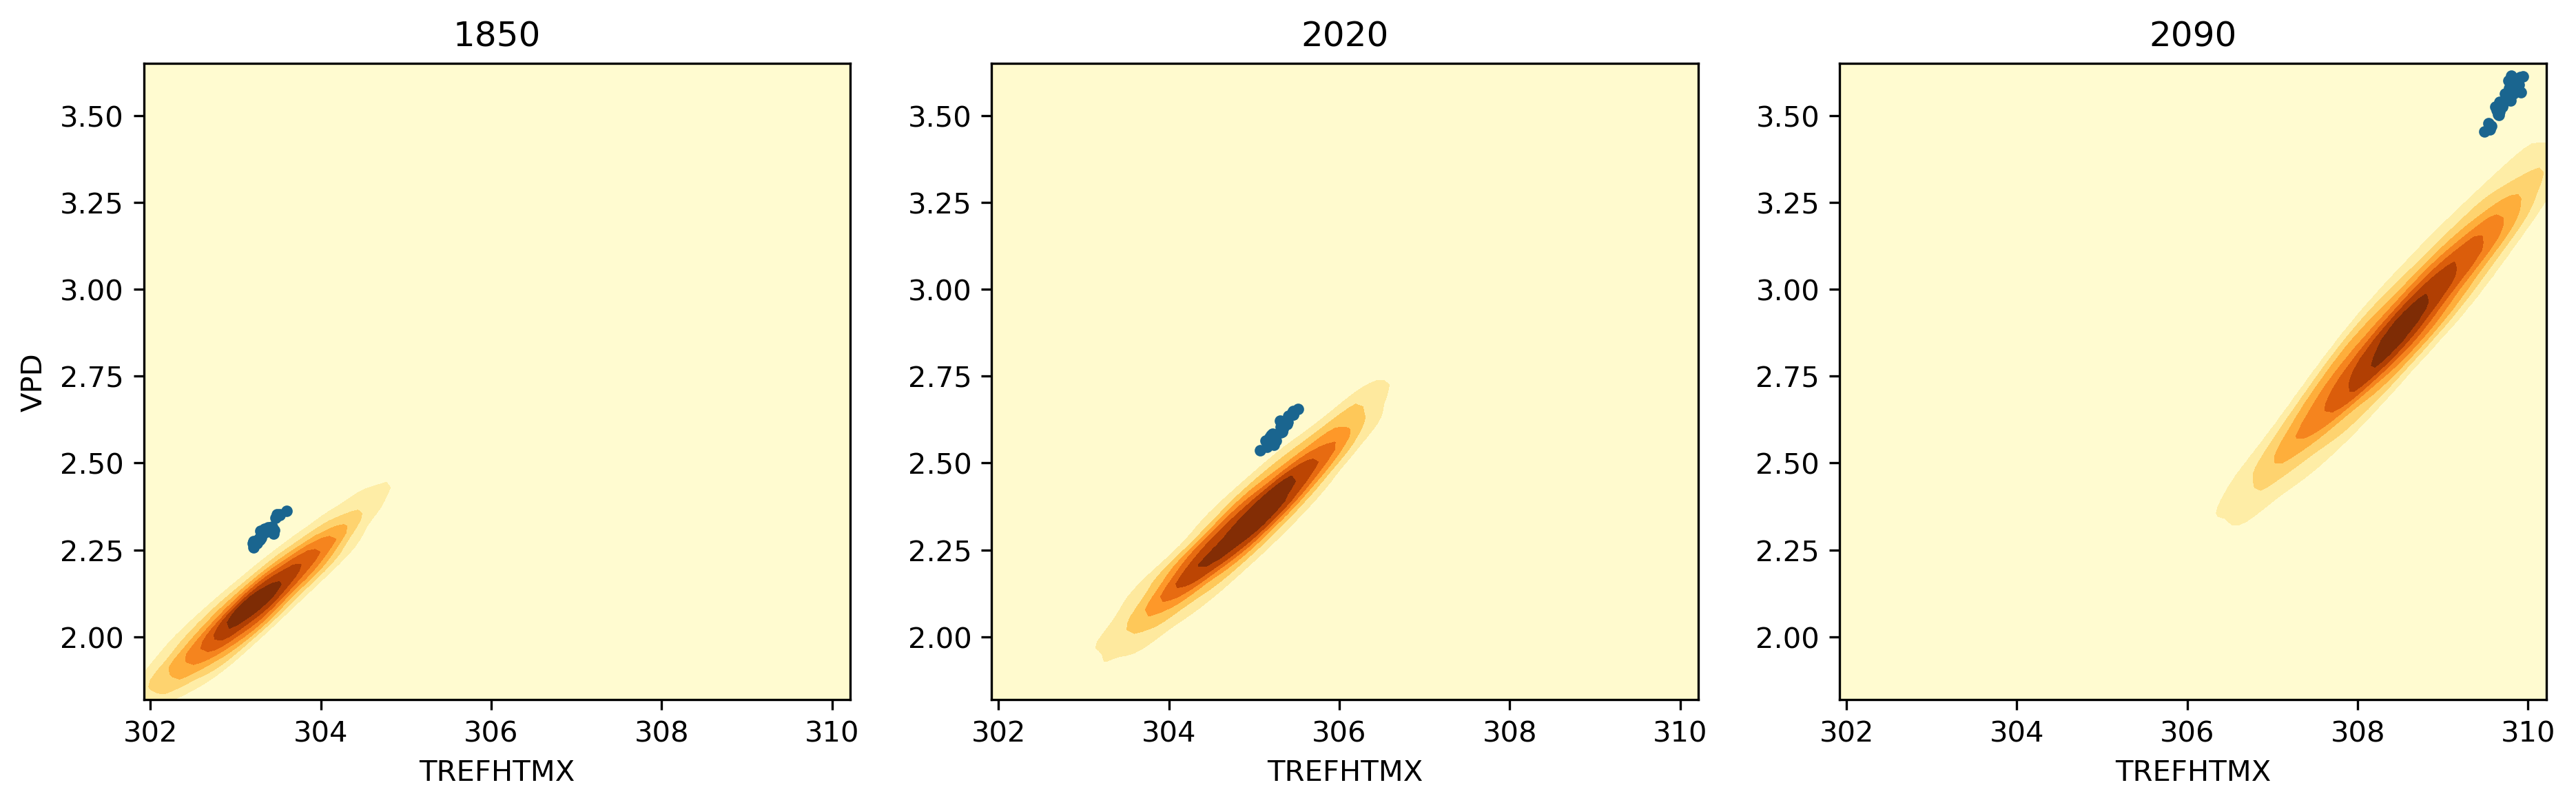
\includegraphics[width=40pc]{figs/contours/TREFHTMX_VPD_contours.png}
\caption{[SUPP] The CCE air is very dry, especially in 2090. Partly due to a stronger warming effect in the CCE than in the coupled model.}
\label{fig:precip}
\end{figure}


\begin{figure}[h]
\centering
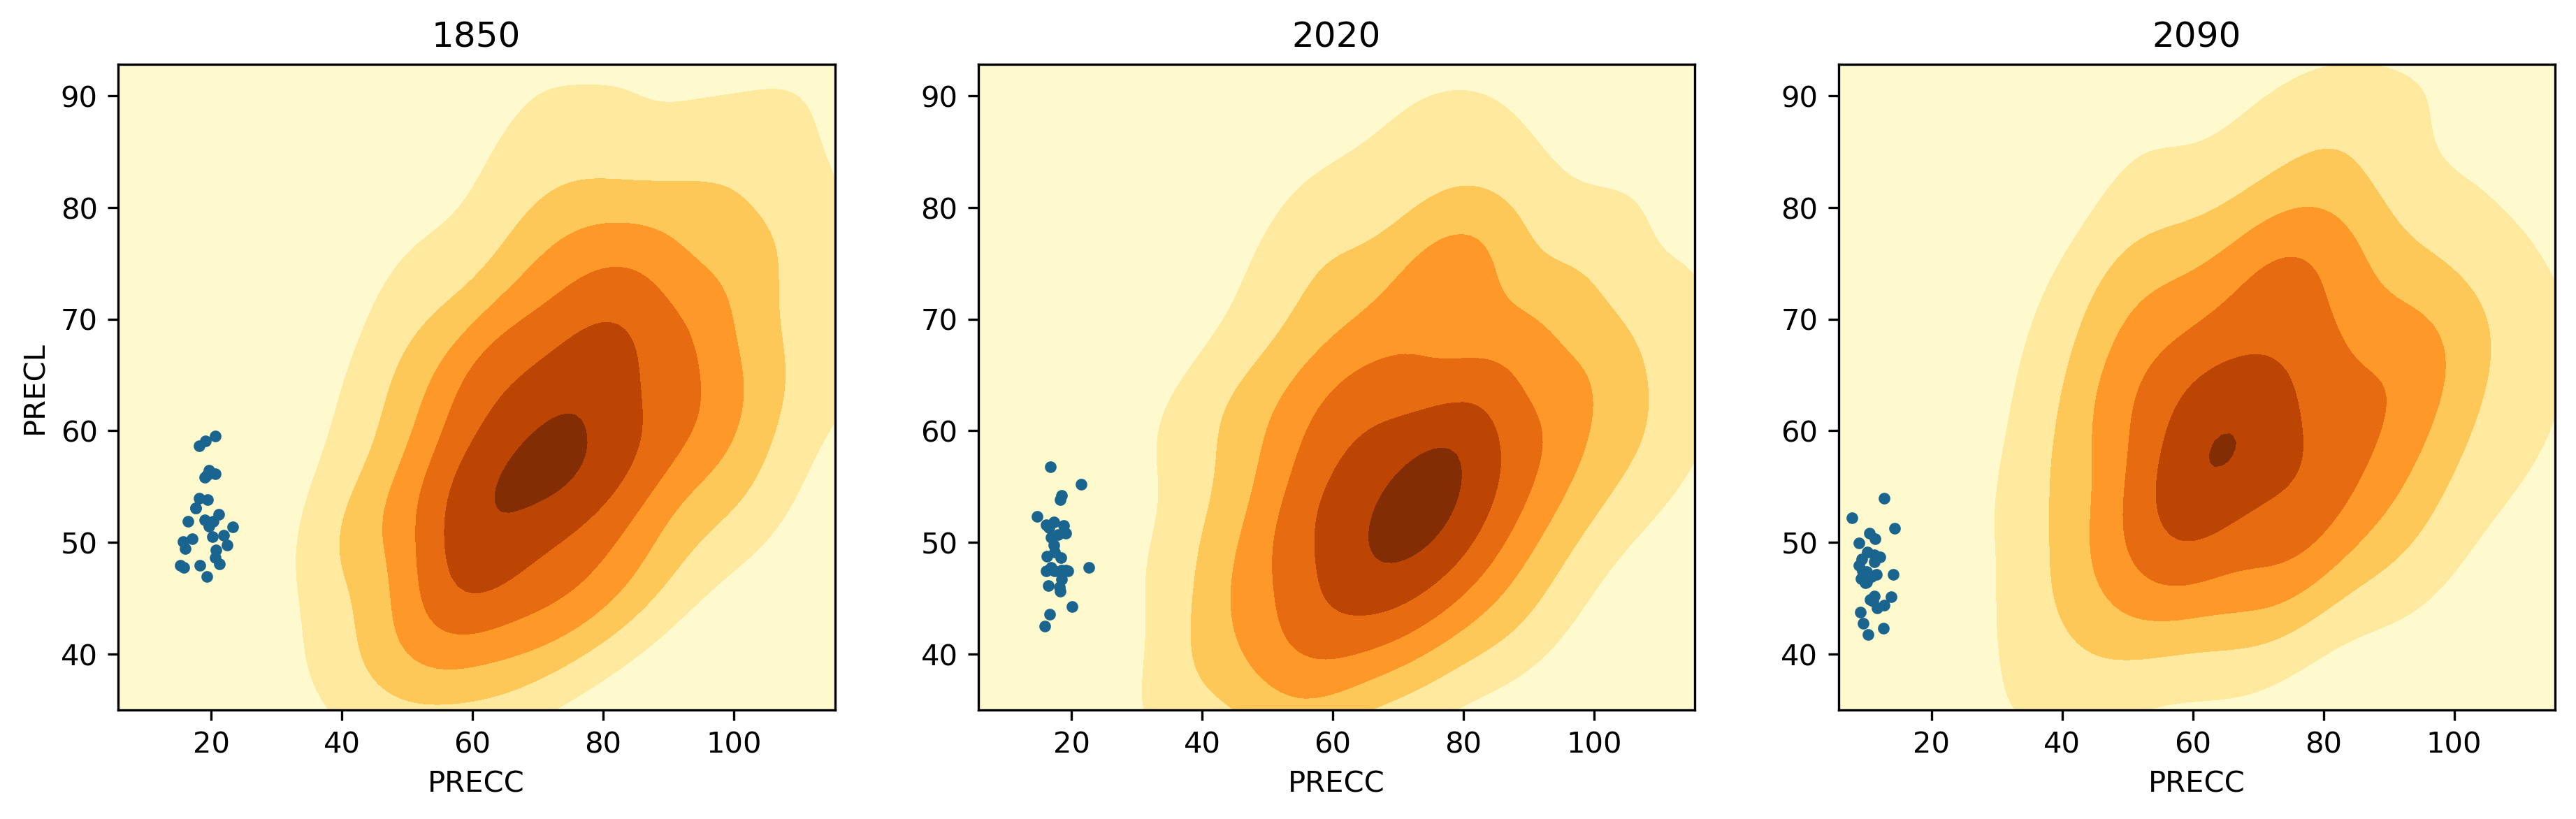
\includegraphics[width=40pc]{figs/contours/PRECC_PRECL_contours.png}
\caption{[SUPP] The CCE is extreme in convective precipitation as opposed to large-scale? Both are decreasing with warming.}
\label{fig:precip}
\end{figure}


\bibliographystyle{abbrvnat}
\nocite{*}
\bibliography{refs/all}
\end{document}




